\documentclass[tikz,border=6pt]{standalone}
% Shared visual language for the book's standalone vector figures.
% Keep this file compatible with the TeX Live version used by LyX.
\usepackage{amsmath,amssymb}
\usepackage{array,booktabs}
\usepackage{pgfplots}
\usepackage{pgfplotstable}
\usetikzlibrary{arrows.meta,calc,positioning}
\pgfplotsset{compat=1.17}

\definecolor{BookBlue}{HTML}{0072B2}
\definecolor{BookOrange}{HTML}{D55E00}
\definecolor{BookGreen}{HTML}{009E73}
\definecolor{BookGray}{HTML}{666666}
\definecolor{BookLightGray}{HTML}{D9D9D9}

\pgfplotsset{
  book axis/.style={
    axis line style={black!75,line width=0.55pt},
    tick style={black!75,line width=0.45pt},
    tick label style={font=\small},
    label style={font=\small},
    legend style={
      font=\small,
      draw=none,
      fill=none,
      cells={anchor=west},
    },
    grid style={BookLightGray,line width=0.35pt},
    major grid style={BookLightGray,line width=0.35pt},
  },
}

\begin{document}
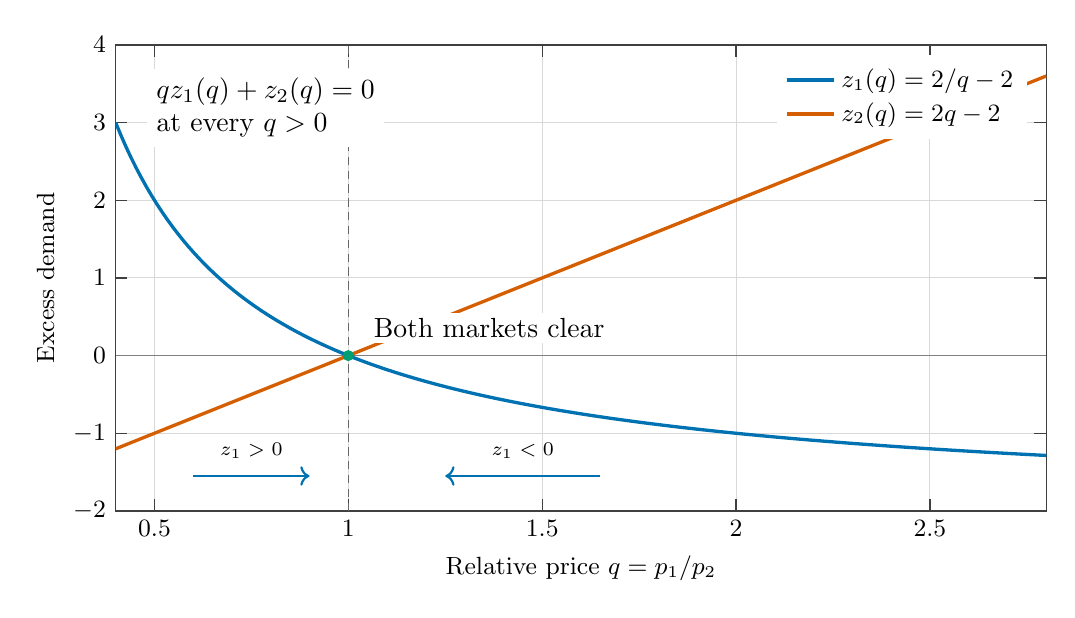
\begin{tikzpicture}
\begin{axis}[book axis,width=13.4cm,height=7.5cm,xmin=.4,xmax=2.8,
 ymin=-2,ymax=4,xlabel={Relative price $q=p_1/p_2$},ylabel={Excess demand},
 xtick={.5,1,1.5,2,2.5},ytick={-2,-1,0,1,2,3,4},grid=major,
 legend style={at={(.98,.98)},anchor=north east,fill=white,
   fill opacity=1,text opacity=1,inner sep=3pt}]
 \addplot[black!50,thin,forget plot,domain=.4:2.8] {0};
 \addplot[BookBlue,very thick,domain=.4:2.8,samples=180] {2/x-2};
 \addlegendentry{$z_1(q)=2/q-2$}
 \addplot[BookOrange,very thick,domain=.4:2.8] {2*x-2};
 \addlegendentry{$z_2(q)=2q-2$}
 \draw[densely dashed,BookGray] (axis cs:1,-2)--(axis cs:1,4);
 \fill[BookGreen] (axis cs:1,0) circle(2pt);
 \node[anchor=south west,fill=white,inner sep=2pt] at(axis cs:1.05,.15){Both markets clear};
 \node[anchor=north west,fill=white,align=left] at(axis cs:.48,3.7)
   {$qz_1(q)+z_2(q)=0$\\at every $q>0$};
 \draw[->,BookBlue,thick] (axis cs:.6,-1.55)--(axis cs:.9,-1.55);
 \draw[->,BookBlue,thick] (axis cs:1.65,-1.55)--(axis cs:1.25,-1.55);
 \node[font=\scriptsize,anchor=south] at(axis cs:.75,-1.45){$z_1>0$};
 \node[font=\scriptsize,anchor=south] at(axis cs:1.45,-1.45){$z_1<0$};
\end{axis}
\end{tikzpicture}
\end{document}
